
\documentclass[final]{beamer}

\usepackage[scale=1.35,size=custom,width=42,height=48]{beamerposter} % Use the beamerposter package for laying out the poster

\usepackage{amsthm}
\usepackage{amsmath}
\usepackage{transparent}
\usepackage{relsize}
\usepackage{lmodern}
\usepackage{exscale}
\usepackage{anyfontsize}
\usepackage{pdfpages}
\usepackage{fontspec}
%\usepackage{parskip}

\usepackage{graphicx, import}  % Required for including images

\usetheme{confposter} % Use the confposter theme supplied with this template

\setbeamercolor{block title}{fg=ngreen,bg=white} % Colors of the block titles
\setbeamercolor{block body}{fg=black,bg=white} % Colors of the body of blocks
\setbeamercolor{block alerted title}{fg=white,bg=dblue!70} % Colors of the highlighted block titles
\setbeamercolor{block alerted body}{fg=black,bg=dblue!10} % Colors of the body of highlighted blocks
% Many more colors are available for use in beamerthemeconfposter.sty

%-----------------------------------------------------------
% Define the column widths and overall poster size
% To set effective sepwid, onecolwid and twocolwid values, first choose how many columns you want and how much separation you want between columns
% In this template, the separation width chosen is 0.024 of the paper width and a 4-column layout
% onecolwid should therefore be (1-(# of columns+1)*sepwid)/# of columns e.g. (1-(4+1)*0.024)/4 = 0.22
% Set twocolwid to be (2*onecolwid)+sepwid = 0.464
% Set threecolwid to be (3*onecolwid)+2*sepwid = 0.708

\newlength{\sepwid}
\newlength{\leftcolwid}
\newlength{\rightcolwid}
\newlength{\twocolwid}
\setlength{\paperwidth}{48in} % A0 width: 46.8in
\setlength{\paperheight}{42in} % A0 height: 33.1in
\setlength{\sepwid}{0.0125\paperwidth} % Separation width (white space) between columns
\setlength{\leftcolwid}{0.285\paperwidth} % Width of one column
\setlength{\twocolwid}{0.38\paperwidth} % Width of two columns
\setlength{\rightcolwid}{0.285\paperwidth} % Width of one column
\setlength{\topmargin}{-0.5in} % Reduce the top margin size

\usepackage{xcolor}
\usepackage{soul}

\newcommand{\hlc}[1]{{%
    \colorbox{yellow}{#1}}%
}

\renewcommand{\baselinestretch}{1.05}
\setbeamertemplate{itemize item}{$\scriptstyle\blacktriangleright$}

%\setmainfont[Ligatures=TeX]{Cambria}

%-----------------------------------------------------------


%----------------------------------------------------------------------------------------
%	TITLE SECTION 
%----------------------------------------------------------------------------------------

\title{Local-Access Generators} % Poster title

\author{Amartya Shankha Biswas, Ronitt Rubinfeld, Anak Yodpinyanee} % Author(s)

\institute{CSAIL, MIT} % Institution(s)

%----------------------------------------------------------------------------------------

\begin{document}


\addtobeamertemplate{block end}{}{\vspace*{2ex}} % White space under blocks
\addtobeamertemplate{block alerted end}{}{\vspace*{2ex}} % White space under highlighted (alert) blocks

\setlength{\belowcaptionskip}{2ex} % White space under figures
\setlength\belowdisplayshortskip{2ex} % White space under equations

\begin{frame}[t] % The whole poster is enclosed in one beamer frame


\begin{columns}[t] % The whole poster consists of three major columns, the second of which is split into two columns twice - the [t] option aligns each column's content to the top

\begin{column}{\sepwid}\end{column} % Empty spacer column

\begin{column}{\leftcolwid} % The first column

\setbeamercolor{block title}{fg=Mahogany,bg=white} % Change the block title color
\begin{block}{Partial Sampling from a Distribution}



\setbeamercolor{block alerted title}{bg=PineGreen} % Change the alert block title colors
\begin{alertblock}{Full Sampling $R \sim\mathsf D$ in $\mathcal O (T)$ time}

\begin{figure}[h!]\centering
    \def\svgwidth{0.5\columnwidth}
    \import{svg/}{generic_sampling.pdf_tex}
\end{figure}

\end{alertblock}


\begin{alertblock}{Do we need to spend $\mathcal{O}(T)$ upfront?}

\begin{center}
\textbf{Partial sampling:} each step should take $\tilde{\mathcal O} (T/N)$ time.
\end{center}

\begin{figure}[h!]\centering
    \def\svgwidth{0.7\columnwidth}
    \import{svg/}{partial_sampling.pdf_tex}
\end{figure}

\end{alertblock}


\setbeamercolor{block alerted title}{bg=Bittersweet} % Change the alert block title colors
\begin{alertblock}{\textbf{Problem Statement}}

A local-access generator of a random object $R \sim\mathsf D$,
provides indirect access to $R'$ with a \emph{query oracle} s.t.
\begin{itemize}
    \item All query responses (\emph{partial samples}) are \textbf{consistent}
    \item The \textbf{distribution} of $R'$ is $\epsilon$-close to $\mathsf D$ in $L_1$ distance
\end{itemize}

\end{alertblock}



\end{block}


\begin{block}{Sampling $G(n, p)$: \textsf{Vertex-Pair} queries}

%\textbf{Model:} $n$-vertex undirected graph: edge probability $p$

\textbf{\textsf{Vertex-Pair}}: Given vertices $u, v$, decide whether $(u,v)\in E$.
%\begin{itemize}
%    \item [] \textbf{Query Model:} Given vertices $u, v$, is $(u,v)\in E$?
    %\item 
    \emph{Trivial}: just a collection of $n \choose 2$ Bernoulli RVs with bias $p$.
%\end{itemize}

\end{block}

\begin{block}{\textsf{Next-Neighbor} queries (skip-sampling)}

\textbf{\textsf{Next-Neighbor}}: Return neighbors of $v$ in order.

\vspace{15pt}


\colorbox{BlueGreen}{\textbf{Na\"ive solution:}} Toss $1/p$ coins until a neighbor is found.

\emph{Idea}: can compute \textsf{Next-Neighbor}'s distribution's CDF from
\vspace{-10pt}
\[ \mathbb P[k \textrm{ non-neighbors before next-neighbor}] = p(1-p)^k \]

\colorbox{BlueGreen}{\textbf{Skip-sampling:}} Draw from \textsf{Next-Neighbor} distribution
\vspace{-20pt}
\begin{itemize}
    \item Can sample from this distribution in $\tilde{\mathcal O}(1)$ time [ELMR17]
    \item Further analysis required for finite-precision arithmetic
%    \item Na\"ive sampling spends $1/p$ time sampling the $0$'s
\end{itemize}

\emph{\color{red}Issue:} Adjacency matrix is symmetric; we need to \textbf{record all generated $0$'s} in the corresponding column of $v$

\begin{figure}[h!]\centering
    \def\svgwidth{0.9\columnwidth}
    \import{svg/}{skip_sampling.pdf_tex}
\end{figure}
\emph{\color{red}Issue:} if the sampled neighbor is already $0$, must re-sample

\quad$\Rightarrow$ may hit $0$'s many times -- \textbf{too many re-samplings}

\end{block}


\end{column} % End of the first column


\begin{column}{\sepwid}\end{column} % Empty spacer column


\begin{column}{\twocolwid} % Begin a column which is two columns wide (column 2)


\setbeamercolor{block title}{fg=Mahogany,bg=white} % Change the block title color
\begin{block}{\textsf{Random-Neighbor} queries (\textsc{Bucketing-Generator})}
\textbf{\textsf{Random-Neighbor}}: Return a neighbor of $v$ uniformly at random.

\vspace{15pt}
\emph{\color{red}Issue:} \textsf{next-neighbor} can't jump to a random potential neighbor of $v$

\colorbox{BlueGreen}{\textbf{Bucketing}} Divide each row of the adjacency matrix into contiguous buckets

\quad$\Rightarrow$ random neighbor of $v\approx$ random neighbor in a random bucket of $v$

\vspace{15pt}

\emph{\color{red}Issue:} do \textbf{not} know $\deg(v)$; must return each neighbor with probability $1/\deg(v)$

\colorbox{BlueGreen}{\textbf{Rejection Sampling}} Return \textbf{any} neighbor with the \textbf{same} probability 

\begin{figure}[h]
    \centering
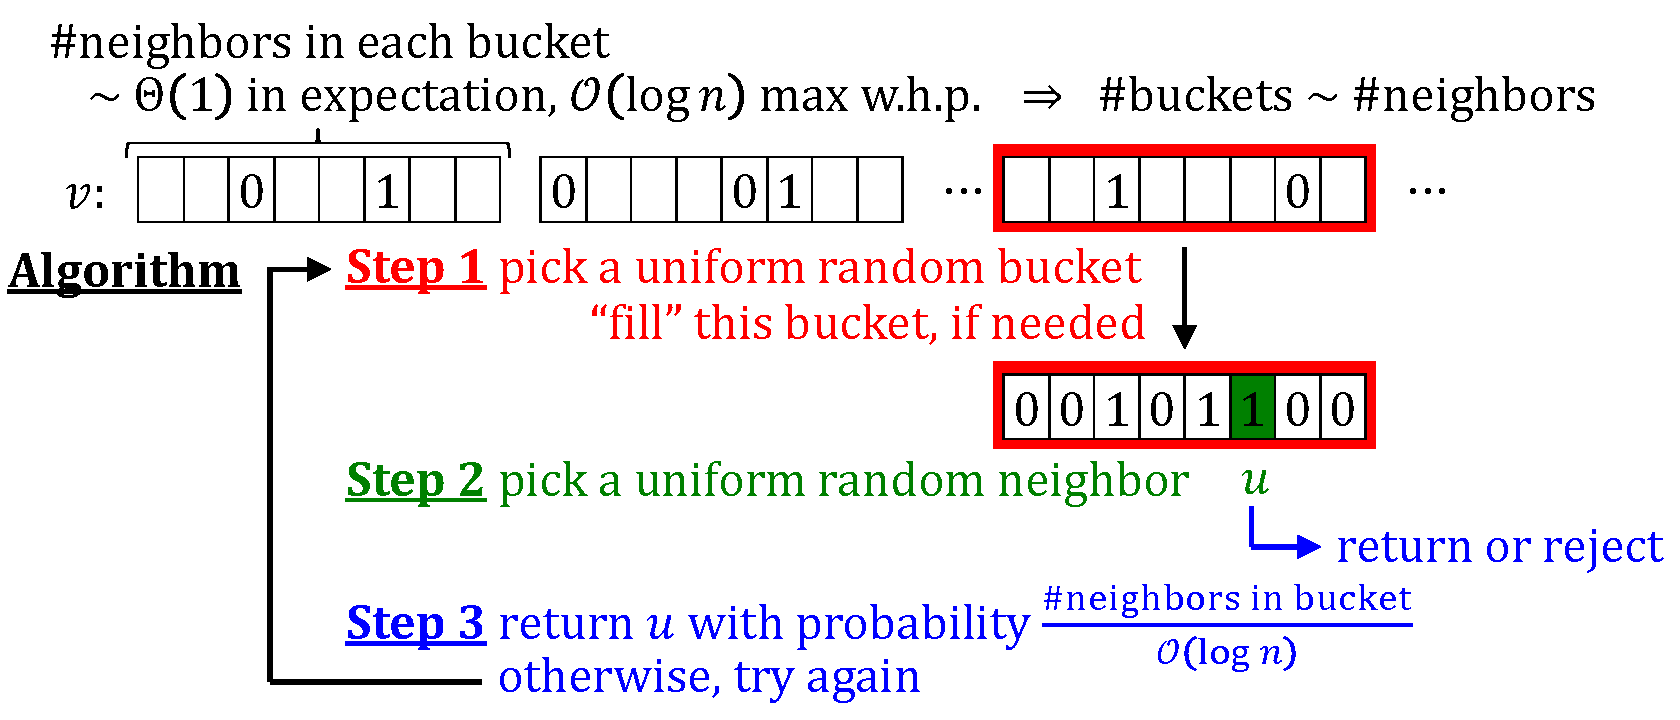
\includegraphics[clip, width=0.95\textwidth]{bckt.pdf}
\end{figure}

$\mathbb P[\textrm{return }u] = {\color{red}\frac{1}{\#\textrm{buckets}}} \times {\color{Emerald}\frac{1}{\#\textrm{neighbors in bucket}}} \times {\color{blue}\frac{\#\textrm{neighbors in bucket}}{\mathcal{O}(\log n)}}\approx\frac{\Omega(1/\log n)}{\#\textrm{neighbors of }v}$

\vspace{5pt}

$\displaystyle\mathbb P[\textrm{return any neighbor}] \approx \Omega(1/\log n) \Rightarrow$ $\mathcal{O}(\log n)$ iterations suffice

\vspace{15pt}
\colorbox{BlueGreen}{\textbf{Data Structure}} bucket maintains its known neighbors and a \textbf{filled} marker
\vspace{-8pt}
\[
  \begin{array}{l}
  \textrm{``fill'' with expected }\mathcal{O}(1)\textrm{ \textsf{Next-Neighbor} queries}\\
  \textrm{\textsf{Random-Neighbor} succeeds in }\mathcal{O}(\log n)\textrm{ tries}
  \end{array}
  \bigg\}
  \begin{array}{l}
  \mathcal{O}(\log n)\textrm{ expected time}\\
  \tilde{\mathcal{O}}(n+m)\textrm{ \emph{total} space usage}
  \end{array}
\]

%Issue: $\textsc{next-neighbor}$ can't jump to a random potential neighbor of $v$
%\begin{itemize}
    %%\item [] \textbf{Bounding the number of re-samplings:}
    %\item Divide each row of the adjacency matrix into contiguous buckets
    %\item Expected number of neighbors in a bucket is $\Theta(\log n)$
    %\item Each vertex $v$ is associated with buckets $ \langle B^v_1, B^v_2, B^v_3,\cdots\rangle$
    %\item An \textbf{unfilled} bucket may contain some indirectly exposed neighbors
    %\item A \textbf{filled} bucket will contain every possible sampled neighbor
%\end{itemize}

%%\setbeamercolor{block alerted title}{bg=Periwinkle} % Change the alert block title colors
%\begin{alertblock}{Filling the $i^{th}$ bucket $B^v_i$ of vertex $v$}
%\begin{itemize}
    %\item Use skip-sampling to produce a \textbf{potential} \emph{next-neighbor} $u$ of $v$ in $B^v_i$
    %\item Check if $(u, v)$ was set to $0$, by looking at bucket $\mathcal B$ of $u$ containing $v$
    %\item If so, re-sample. Otherwise, mark $u$ as a neighbor of $v$, and update $\mathcal B$
    %\item W.h.p, only $\mathcal O(\log^2 n)$ \textbf{potential} neighbors are generated in $B^v_i$
    %%\item With high probability, none of the buckets contain zero neighbors.
%\end{itemize}
%\end{alertblock}

\end{block}



%\vspace{-0.5in}
%%\begin{columns}[t,totalwidth=\twocolwid]

%%\begin{column}{0.49\twocolwid}

%\begin{itemize}
    %\item [] \textbf{Degree Sampling:} Sampling the degree of $v$ seems to be much harder
    %\item Sampling $deg(v)$ conditions the remaining RVs in very non-trivial ways
    %\item However, we can stil sample a random neighbor (with prob. $1/deg(v)$)
%\end{itemize}

%%\setbeamercolor{block alerted title}{bg=Periwinkle} % Change the alert block title colors
%\begin{alertblock}{$\textsc{Random-Neighbor}(v)$}
%\begin{itemize}
    %\item Choose a random bucket $\mathcal B$ of $v$. If the $\mathcal B$ is \textbf{unfilled}, fill it.
    %\item If $k$ neighbors found in $\mathcal B$, start over (reject) with probability $1-k/M$.
    %\item If accepted, return an uniformly random neighbor found in $\mathcal B$.
%\end{itemize}
%For $M = \mathcal O(\log^2 N)$, the max number of neighbors in any bucket is $<M$.
%So, the number of rejection sampling rounds is $\mathcal O(\log^2 N)$ in expectation.
%\end{alertblock}

\vspace{-0.3em}
\begin{block}{Stochastic Block Model}%: Random Community Assignment}

%\begin{itemize}
    %\item Each vertex is assigned to some community $C_i\subseteq V$ for $i\in [r]$
Communities $\{C_i\}_{i\in [r]}$ partition $V$: If $u\in C_i, v\in C_j$, then $\mathbb P_{(u, v)\in E} = p_{ij}$.
    %where $\left\{ p_{ij}\right\}_{i,j\in [r]}\in [0,1]^{r\times r}$
%\end{itemize}
\begin{itemize}
\item [] \textbf{Given sizes of each comunity $C_i$ and a range of length $\ell$}
    \item Count number of occurrences of each community in any contiguous range%: $|[a,b]\cap C_j|$
    \item Sample from \emph{Multivariate Hypergeometric Distribution}%: $O(r\, poly(\log n))$ resources
\[
\Pr[\mathbf{S}^\mathbf{C}_\ell = \langle s_1, \ldots, s_r \rangle]
= \frac{\binom{C_1}{s_1}\cdot\binom{C_2}{s_2}\cdots\binom{C_r}{s_r}}{\binom{B}{\ell}}
\hspace{2ex}\textrm{ where } \scriptstyle{
    \ell = \mathlarger{\sum}\limits^{r}_{i=1} s_i \textrm{ and } B = \mathlarger{\sum}\limits^{r}_{i=1} C_i
}
\]
\end{itemize}

\begin{figure}[h!]\centering
    \def\svgwidth{0.8\columnwidth}
    \import{svg/}{counting.pdf_tex}
\end{figure}


\end{block}



\end{column} % End of the second column



\begin{column}{\sepwid}\end{column} % Empty spacer column



\begin{column}{\rightcolwid} % The third column

\setbeamercolor{block alerted title}{bg=CadetBlue} % Change the alert block title colors
\begin{alertblock}{Multivariate Hypergeometric Distribution}
[GGN10] solves the special case of $r=2$ and $B = 2\ell$.
\begin{itemize}
    \item [] $\textsc{Counting-Generator}$
    \item \textbf{Extending to $B\not= 2\ell$}: Divide $\ell$ into dyadic segments.
    \item \textbf{Extending to $r>2$}: Make a tree with a leaf for each $C_i$
          Every branch in the tree is equivalent to a $2$-splitting
\end{itemize}
\end{alertblock}

\begin{itemize}
    \item Use $\textsc{Counting-Generator}$ to sample community counts
    \item Run the $\textsc{Bucketing-Generator}$ as before
\end{itemize}



\setbeamercolor{block title}{fg=Mahogany,bg=white} % Change the block title color
\begin{block}{Work in Progress}



\setbeamercolor{block alerted title}{bg=norange} % Change the alert block title colors
\begin{alertblock}{Domino Tiling}
A $2\times n$ grid tiled with dominoes: $F_n$ tilings possible.
\begin{figure}[h!]\centering
    \def\svgwidth{0.8\columnwidth}
    \import{svg/}{domino_tiling.pdf_tex}
\end{figure}
\textbf{Query:} Domino at position $i$: \emph{vertical} OR \emph{horizontal}?
\begin{figure}[h!]\centering
    \def\svgwidth{0.8\columnwidth}
    \import{svg/}{domino_partial.pdf_tex}
\end{figure}
Sufficent to approximate $F_c/F_{c-1}$: Use $\phi$ if $c = \Omega(\log(n))$
\textbf{Open:} $k\times n$ grid for $k = \omega(1)$ and Dimer model.
\end{alertblock}


\begin{alertblock}{Graph Coloring: Glauber Dynamics}
Find random $k$-coloring for graph with max degree $\Delta$
\begin{itemize}
    \item [] \textbf{Global Algorithm} (for $k > 2\Delta$)
    \item Sample $\mathcal O(n\log n)$ (vertex, color) pairs:
          $\left\{ (v_1, c_1), (v_2, c_2), (v_3, c_3), \cdots, (v_r, c_r)\right\}$
    \item For steps $i\in [1\cdots r]$
    \begin{itemize}
        \item If no neighbor of $v_i$  has color $c_i$ set $v_i$'s color to $c_i$.
        \item Else, do nothing
    \end{itemize}
\end{itemize}
\begin{itemize}
    \item [] \textbf{Local Algorithm} (for $k = \Theta(\Delta\log n)$)
    \item Given $v$, what is $color(v)$ (in some random coloring)?
    \item Locally sample occurences of $(v, \star)$ using the \emph{Count Splitting Generator}
    \item Sample $(w, \star)$ if necessary, where $w$ is neighbor of $v$
    \item Query tree is bounded for $k = \Theta(\Delta\log n)$
\end{itemize}
\end{alertblock}


\begin{alertblock}{Dyck Paths}
\end{alertblock}



\end{block}



\end{column} % End of the third column


\end{columns} % End of all the columns in the poster




\begin{column}{0.7\paperwidth}

\let\thefootnote\relax\footnotetext{
    \scriptsize{
        [ELMR17] Guy Even, Reut Levi, Moti Medina, and Adi Rosen.
        Sublinear random access generators for preferential attachment graphs.
        In 44th International Colloquium on Automata, Languages, and Programming,
        ICALP 2017, July 10-14, 2017%, pages 6:1-6:15.
    }
}
\let\thefootnote\relax\footnotetext{
    \scriptsize{
        [GGN10] Oded Goldreich, Shafi Goldwasser, and Asaf Nussboim.
        On the implementation of huge random objects.
        SIAM Journal on Computing, 39(7):2761–2822, 2010.
    }
}

\end{column}



\end{frame} % End of the enclosing frame




\end{document}
